% ---- figure comparaison_distances_line_graphes_cellules_k_2x50
%\begin{figure}[htb!] 
%\centering
%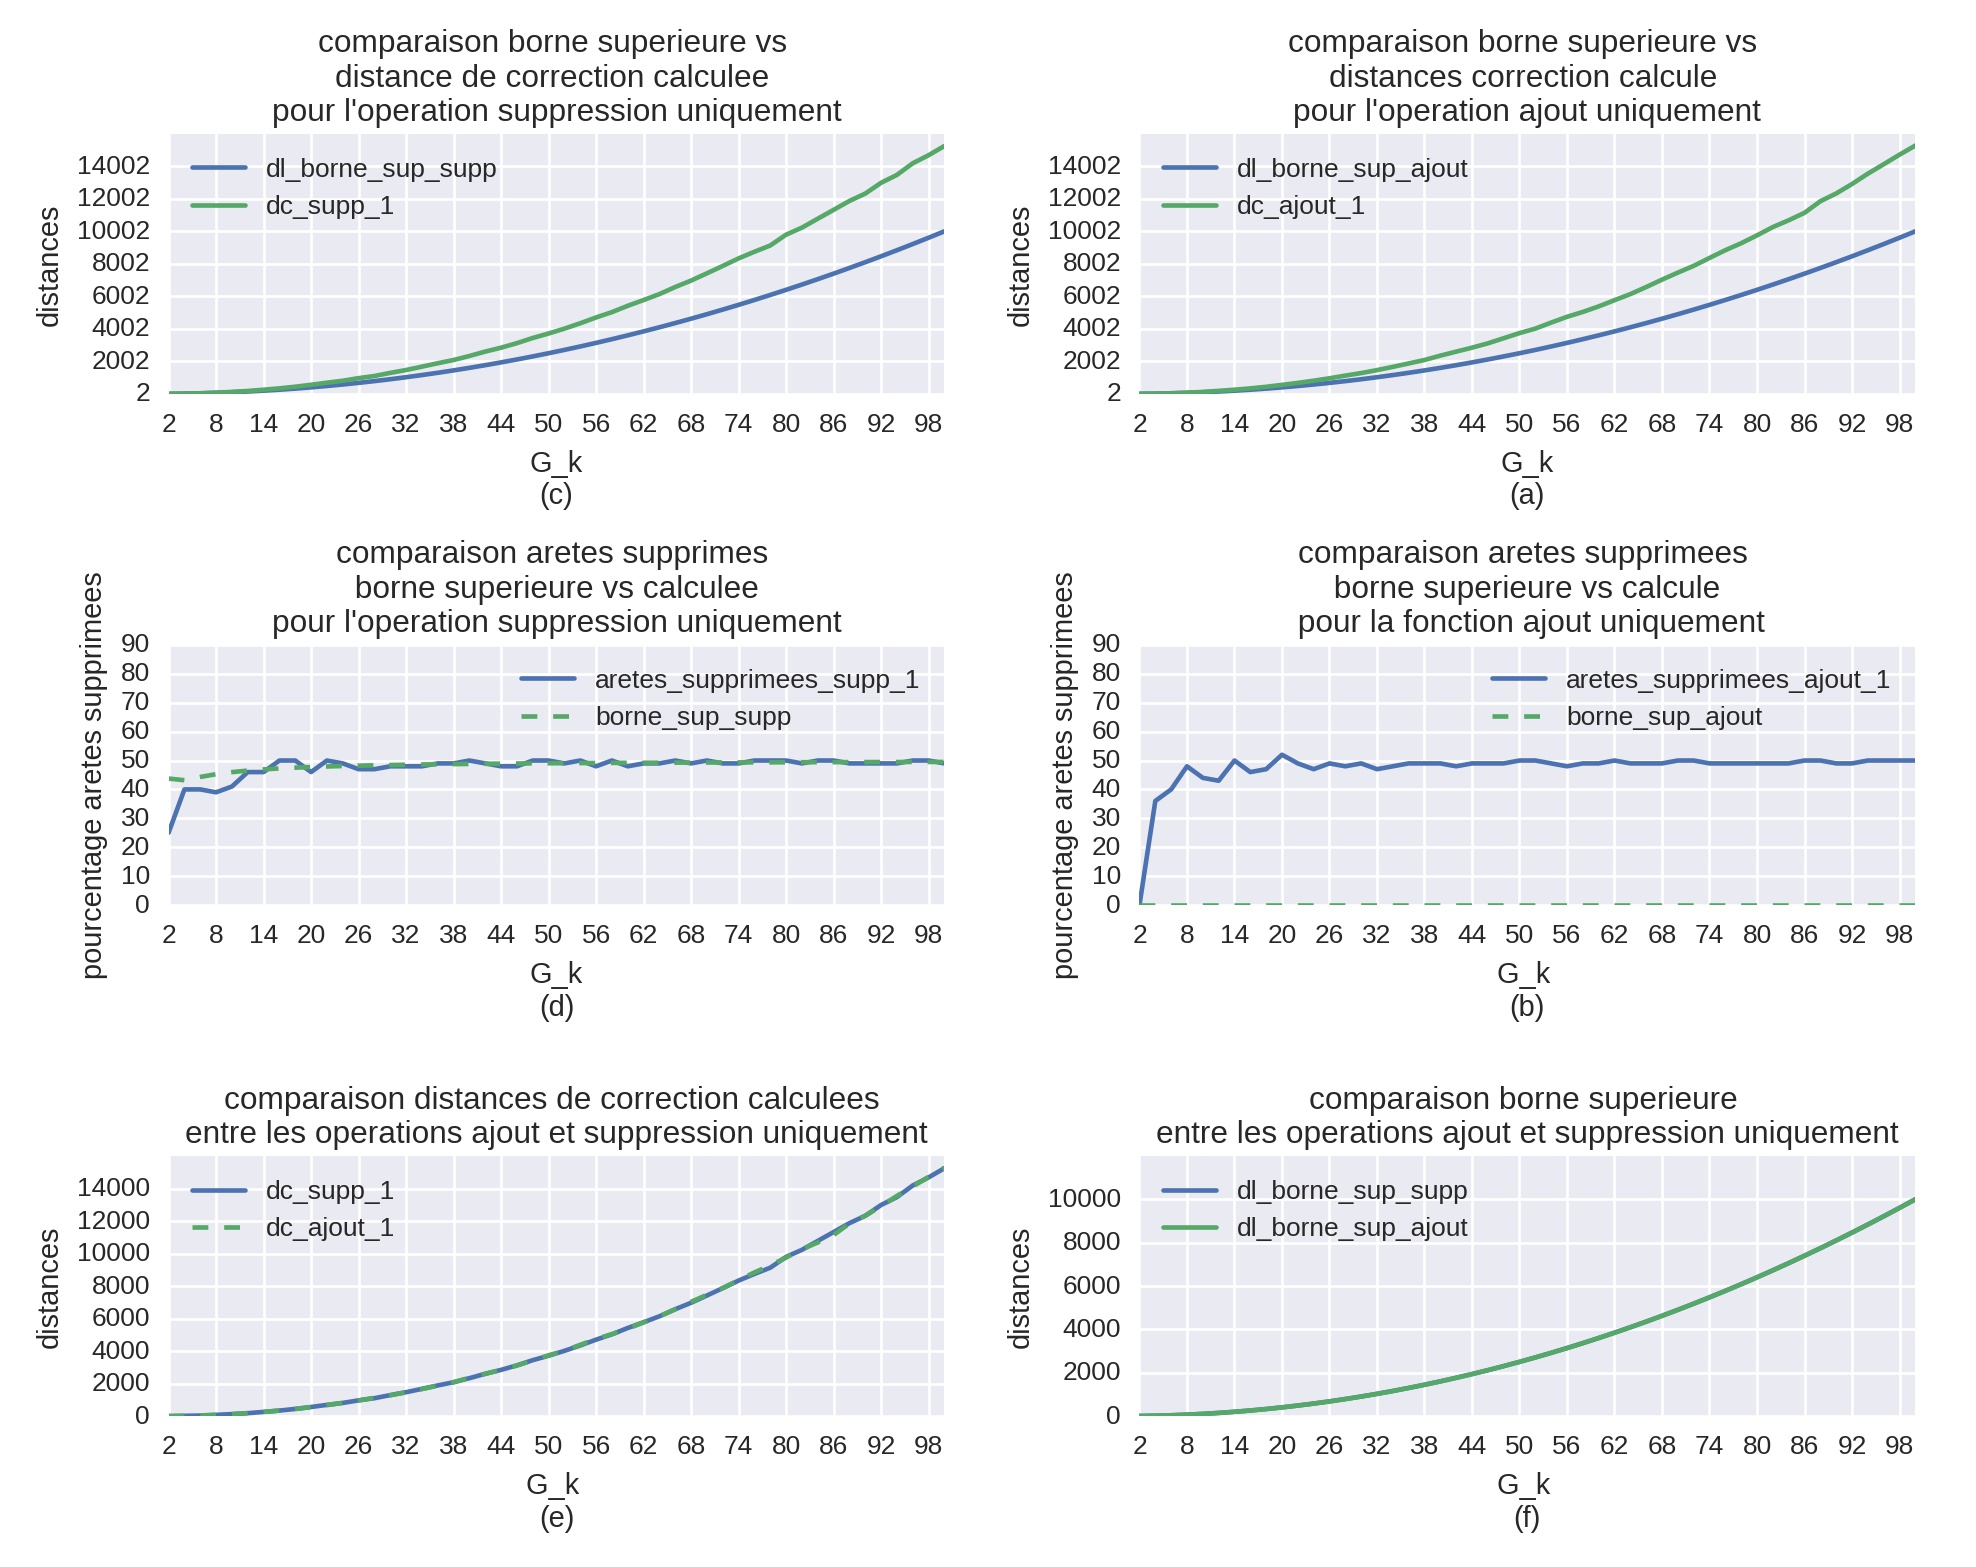
\includegraphics[scale = 0.25]{comparaison_distances_line_graphes_cellules_k_2x50.jpeg}
%\caption{Comparaison de distances lines th\'eoriques et calcul\'ees selon des fonctions de co\^ut {\em suppression} et  {\em ajout}.
%La figure $(a)$ d\'esigne la comparaison entre les distances de correction et la borne sup\'erieure de l'\'equation \ref{borneSuperieureDL} avec la modification {\em ajout d'ar\^etes uniquement}, 
%La figure $(c)$ d\'esigne la comparaison entre les distances de correction et la borne sup\'erieure de l'\'equation \ref{borneSuperieureDL} avec la modification {\em suppression d'ar\^etes uniquement}, 
%La figure $(b)$ compare le pourcentage d'ar\^etes supprim\'ees  dans les graphes boucl\'ees avec celui de la borne sup\'erieure de l'\'equation \ref{borneSuperieureDL} dans la modification {\em ajout d'ar\^etes uniquement}, 
%La figure $(d)$ compare le pourcentage d'ar\^etes supprim\'ees  dans les graphes boucl\'ees avec celui de la borne sup\'erieure de l'\'equation \ref{borneSuperieureDL} dans la modification {\em suppression d'ar\^etes uniquement},
%La figure $(e)$ compare les distances de correction entre les diff\'erentes modifications.
%}
%\label{comparaison_distances_line_graphes_cellules_k_2x50}
%\end{figure}
%\FloatBarrier
\begin{figure}[htb!] 
\centering
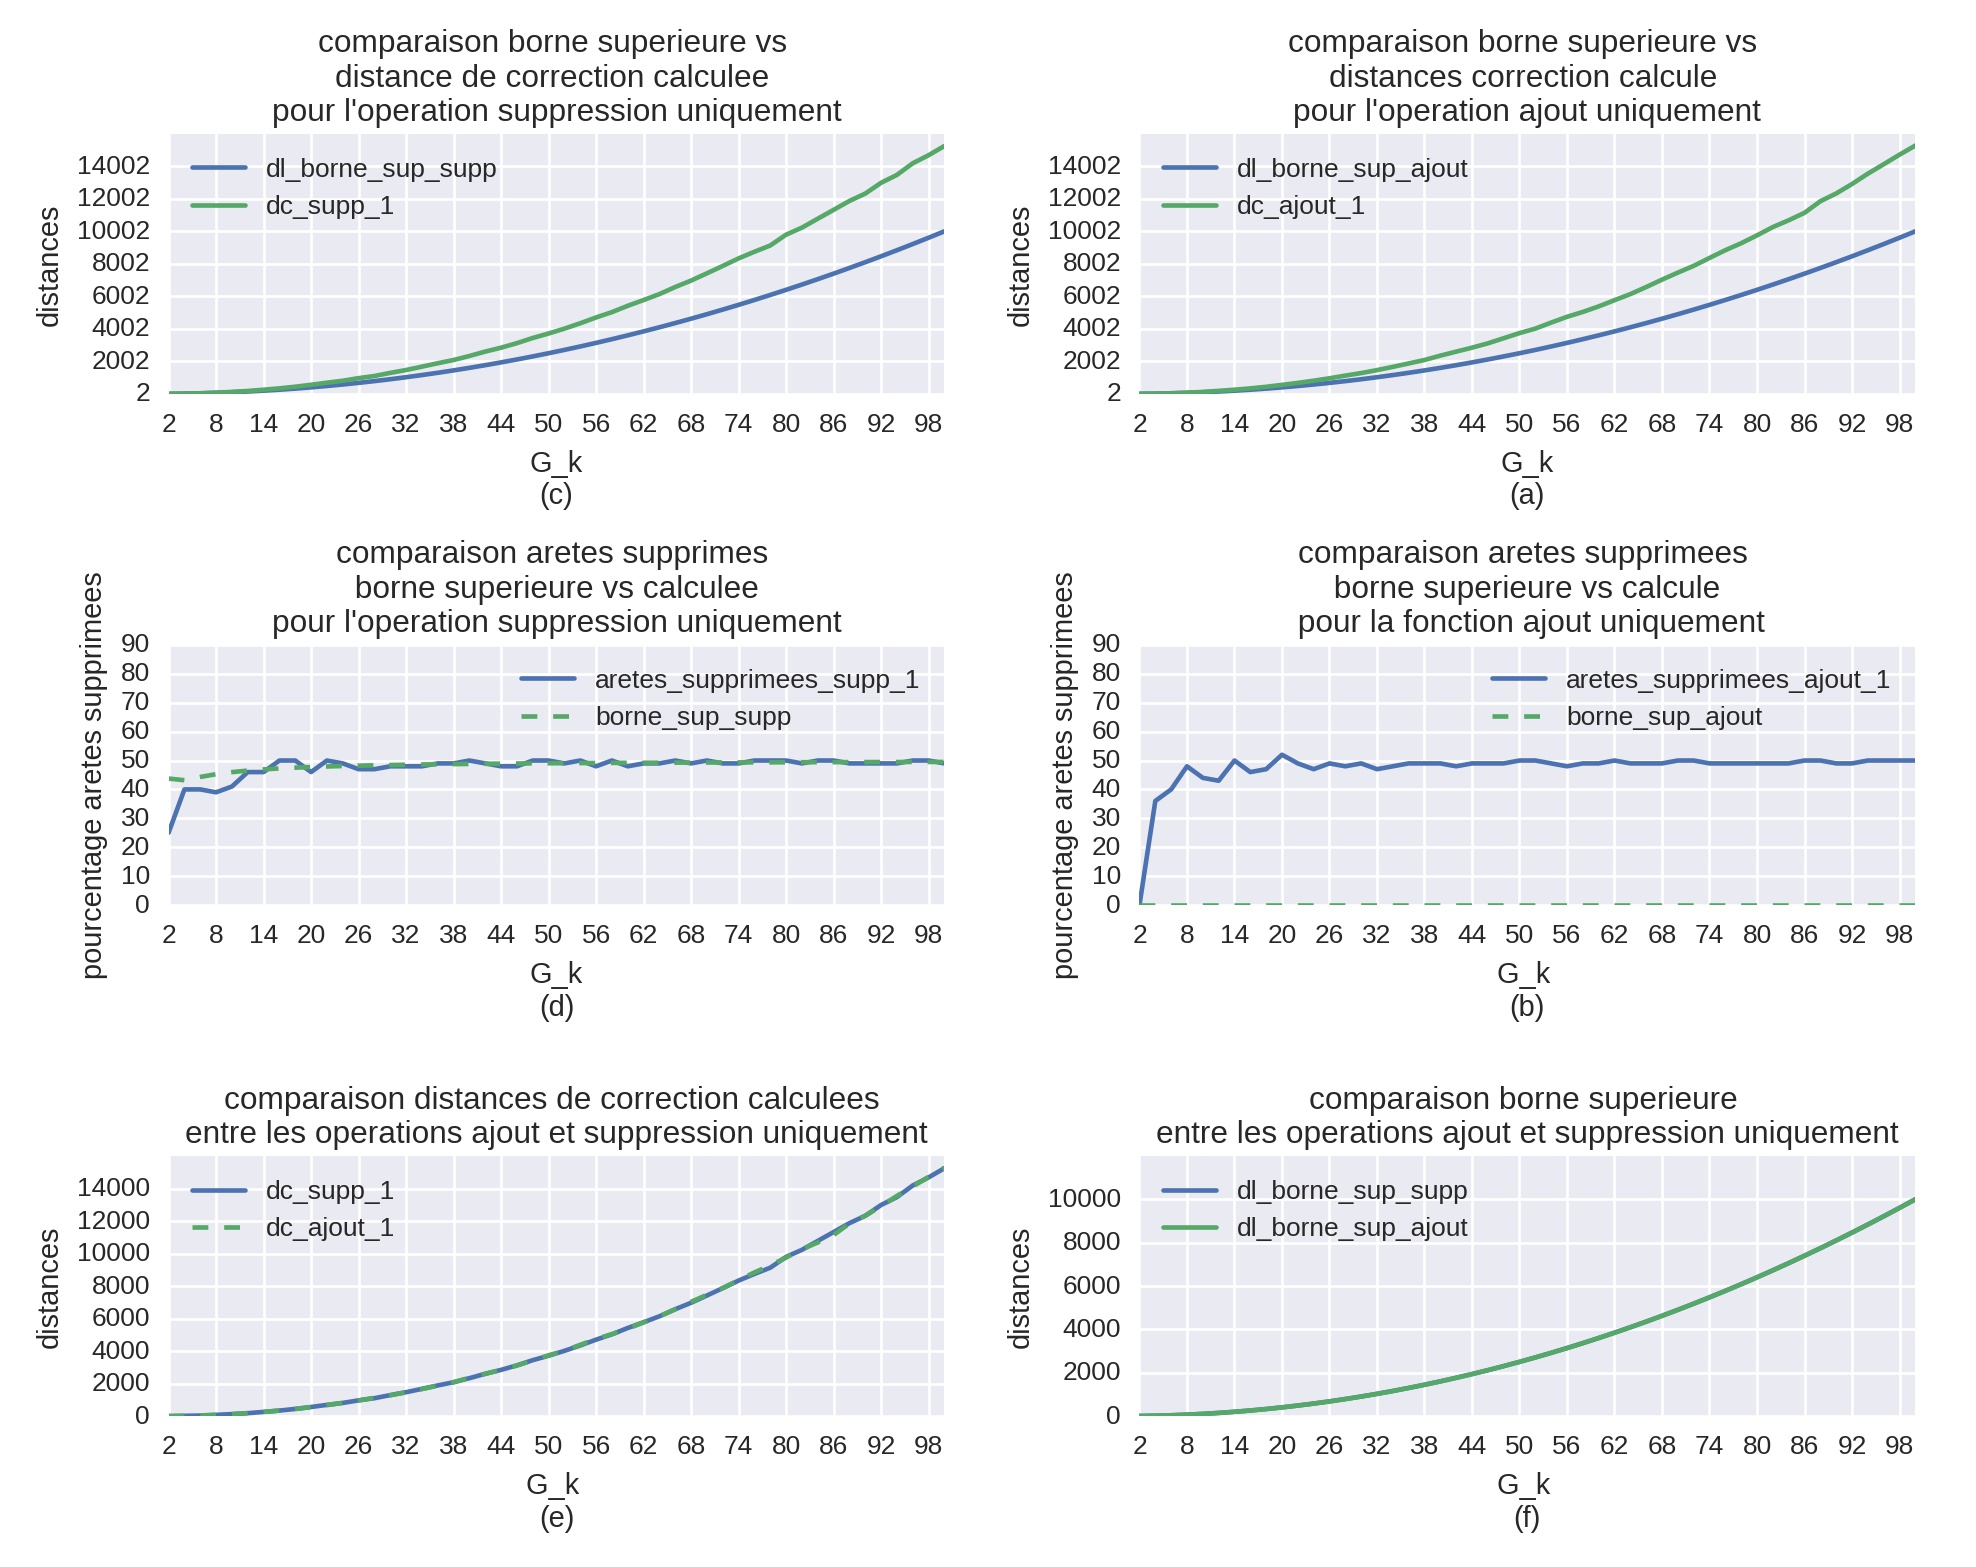
\includegraphics[scale = 0.25]{comparaison_distances_line_graphes_cellules_k_2x50.jpeg}
\caption{Comparaison entre la borne sup\'erieure de la distance line et les distances de correction calcul\'ees selon des fonctions de co\^ut {\em suppression} et  {\em ajout} : 
la figure $(a)$ d\'esigne la comparaison entre les distances de correction et la borne sup\'erieure de l'\'equation \ref{borneSuperieureDL} avec la modification {\em ajout d'ar\^etes uniquement}, 
la figure $(c)$ d\'esigne la comparaison entre les distances de correction et la borne sup\'erieure de l'\'equation \ref{borneSuperieureDL} avec la modification {\em suppression d'ar\^etes uniquement}, 
la figure $(b)$ compare le pourcentage d'ar\^etes supprim\'ees  dans les graphes boucl\'ees avec celui de la borne sup\'erieure de l'\'equation \ref{borneSuperieureDL} dans la modification {\em ajout d'ar\^etes uniquement}, 
la figure $(d)$ compare le pourcentage d'ar\^etes supprim\'ees  dans les graphes boucl\'ees avec celui de la borne sup\'erieure de l'\'equation \ref{borneSuperieureDL} dans la modification {\em suppression d'ar\^etes uniquement},
la figure $(e)$ compare les distances de correction entre les diff\'erentes modifications.
}
\label{comparaison_distances_line_graphes_cellules_k_2x50}
\end{figure}
%\FloatBarrier
% ---- figure comparaison_distances_line_graphes_cellules_k_2x50


Notre objectif est de pr\'esenter les variations des distances de correction par rapport \`a la borne sup\'erieure de la distance line pour chaque modification r\'ealis\'ee sur les graphes pendant l'algorithme de correction. Pour ce faire, nous regroupons notre analyse en $5$ exp\'erimentations.
\newline

Les deux premi\`eres exp\'erimentations comparent les distances de correction avec la borne sup\'erieure pour la modification {\em ajout d'ar\^etes uniquement} (figure \ref{comparaison_distances_line_graphes_cellules_k_2x50} (a) et 
pour la modification {\em suppression d'ar\^etes uniquement} figure \ref{comparaison_distances_line_graphes_cellules_k_2x50} (c).
Nous constatons que les courbes des distances de correction et celle de la borne sup\'erieure sont croissantes. 
La courbe de la borne sup\'erieure, d\'esign\'ee par $borneSup$ dans les graphiques $(a)$ et $(c)$, \'evolue lentement par rapport aux courbes des distances et l'\'ecart entre ces courbes croit lin\'eairement. 
Pour comprendre cet \'ecart croissant, nous v\'erifions le pourcentage d'ar\^etes  supprim\'ees pour chaque modification.  Ce sont les deux autres exp\'erimentations faites et repr\'esent\'ees par la figure 
\ref{comparaison_distances_line_graphes_cellules_k_2x50} (b) pour la modification {\em ajout d'ar\^etes uniquement} et
 la figure \ref{comparaison_distances_line_graphes_cellules_k_2x50} (d) pour la modification 
{\em suppression d'ar\^etes uniquement}. 
En effet, nous avons choisi les ar\^etes supprim\'ees parce que le nombre d'ar\^etes est d\'ej\`a connu c'est-\`a-dire $0$ pour l'ajout uniquement et la borne sup\'erieure pour la suppression uniquement. 
\newline
Nous remarquons que les ar\^etes   de $G_k$ supprim\'ees avoisinent en moyenne de
$40\%$ quand le nombre $k$ de cellules est faible ($k \le 14$) dans la modification {\em ajout ar\^etes uniquement}. Au d\'el\`a de $ k > 14 $, une ar\^ete sur deux du graphe $G_{k}$ est supprim\'ee. La courbe  $aretes\_supprimees\_ajout\_1$ dans le graphique $(b)$ repr\'esente le pourcentage d'ar\^etes supprim\'ees.  
En effet, nous expliquons ces chiffres  par l'ajout d'ar\^etes entre des sommets de cellules voisines et ces sommets ne sont pas partag\'es entre les cellules voisines. Ces ar\^etes ajout\'ees impliquent la suppression des ar\^etes de $G_k$ parce que la partition $\pi_s$ (voir section \ref{algorithmeCorrection}) des ar\^etes \`a supprimer pendant la compression n'est pas vide et contient des ar\^etes de $G_k$ en g\'en\'eral. Ainsi ces ar\^etes provoquent l'abandon des ar\^etes diagonales  ajout\'ees \`a partir du sommet commun entre des cellules comme indiqu\'e dans l'exemple du graphe $G_{4,4}$ dans la figure \ref{exempleCorrectionGrapheCelluleAvecAjout}.
\newline
En ce qui concerne la modification {\em suppression d'ar\^etes uniquement}, les ar\^etes supprim\'ees proviennent aussi des cellules voisines. 
Dans les cellules partageant un sommet, l'algorithme ajoute g\'en\'eralement une ar\^ete diagonale \`a partir de ce sommet commun dans une seule cellule. Les ar\^etes diagonales ajout\'ees sont responsables de l'augmentation de la distance de correction (courbe {\em dc\_supp\_1} dans le graphique $(c)$).
Pour des cellules partageant une ar\^ete, l'algorithme supprime certaines ar\^etes communes comme indiqu\'e dans la section \ref{modificationSuppressionAretesUniquement}. Les autres ar\^etes communes non supprim\'ees sont dues \`a la pr\'esence des ar\^etes diagonales. Cela explique pourquoi nous avons en moyenne $50\%$ des ar\^etes de $G_k$ qui sont supprim\'ees dans le graphique $(d)$. Ce pourcentage est identique \`a celui des ar\^etes supprim\'ees de la borne sup\'erieure lorsque le nombre de cellules devient \'elev\'e $k \ge 18$ et il ne signifie pas que l'algorithme de correction supprime les ar\^etes de la section \ref{modificationSuppressionAretesUniquement}.
\newline
Par ailleurs, les courbes {\em dc\_ajout\_1} de la modification d'{\em ajout d'ar\^etes uniquement} et celle {\em dc\_supp\_1}  de la modification {\em suppression d'ar\^etes uniquement} ont les m\^emes tendances et sont superpos\'ees (figure $(e)$) parce que  dans la modification d'{\em ajout}, l'algorithme ajoute la m\^eme proportion d'ar\^etes qu'il supprime dans  la modification {\em suppression}. 
\newline

\vspace{-0.25cm}
{\bf Conclusion} :   
l'exp\'erimentation montre que le line-graphe $L(G_k)$ propos\'e par l'algorithme de correction pour un $k$ donn\'ee est identique en terme de distance de correction quelle que soit la modification r\'ealis\'ee comme illustre la figure \ref{comparaison_distances_line_graphes_cellules_k_2x50}(e).
Toutefois, les graphes corrig\'es ne sont pas optimaux en terme de distances de correction parce que l'algorithme priorise dans certains cas les modifications {\em ajout d'ar\^etes uniquement} et {\em suppression uniquement} et cela leur permet d'atteindre des minimums locaux. Cependant le minimum global n'est pas atteint g\'en\'eralement. 

